\documentclass[UTF8]{ctexart}
\usepackage{geometry}
\usepackage{amsmath}
\usepackage{lmodern}
\usepackage{graphicx} %插入图片的宏包
\usepackage{float} %设置图片浮动位置的宏包
\geometry{a4paper,scale=0.8}
\sectionfont{\bfseries\Large\raggedright}

\title{deep-learning笔记}
\author{徐世桐}
\date{}
\begin{document}
\maketitle

% --------------------------------------------------------------------------
% |                                基本定义                                  |
% --------------------------------------------------------------------------
\section{基本定义}

\noindent \textbf{label标签}:输出结果,$\hat{y} $为计算得到的结果,$y$为实际测量结果\\
\textbf{feature特征}:用于预测标签的输入变量,$x^{(i)}_j$为第i组sample第j号特征\\
\textbf{sample样本}:一组特征的取值和对应的标签输出\\
\textbf{batch}:batch size个sample被分为一组,进行向量化的计算,称$B$\\
\textbf{hyperparameter超参数}:人为设定的参数。如样本个数(批量大小batch size)$|B|$,学习率$\eta $。少数情况下通过学习得到\\
\textbf{W 一层layer的权重矩阵}:行数 = 前层节点数,列数 = 当前层节点数\\
\textbf{全连接层fully-connected layer/稠密层dense layer}:此层所有节点都分别和前一层所有节点连接\\
\textbf{sigmoid函数}:$\sigma(x) = \frac{1}{1+e^{-x}}$\\
\textbf{softmax函数}:$softmax(Y) = \frac{exp(y)}{\sum_{y' \in Y} exp(y') } $,将数值输出转化为概率值,1. 值为正\ 2. 值总和为1\\
\textbf{cross entropy交叉熵}

  定义:分部p\ 和\ 分部q\ 间的\ cross entropy $H(p, q) = -E_p(\log (q))$。为\ expected value of $log (q)$ with respect to distribution p

  公式:$H(y^{(i)}, \hat{y}^{(i)}) = -\sum_{j\in B}y^{(i)}log(\hat{y}^{(i)})$

  使用:联系两个值概率分部间的差异,即可将数值输出$\hat{y}$和分类结果$y$直接做对比

  \quad 仍可和softmax同时使用,softmax将可能性先转换为正数并和为1,随后使用cross entropy\\
\textbf{指数加权移动平均}

  $y_t = \gamma y_{t-1}+(1-\gamma)x_t$\\
\textbf{小批量乘法}

  对$n$个形状为$(a, b)$矩阵$X_1, X_2, ..., X_n$,$n$个形状为$(b, c)$矩阵$Y_1, Y_2, ..., Y_n$,小批量乘法结果为$X_1Y_1, X_2Y_2, ..., X_nY_n$

  * 特指被word2vec使用的乘法,其他模型仍根据矩阵乘法,非所有批量乘法都使用\ 小批量乘法\\
\textbf{二元交叉熵损失函数}

  得到向量$P = [p_1, ..., p_n]$,向量$L = [l_1, ..., l_n]$,掩码向量$M = [m_1, ..., m_n]$

  \quad $p_i$标记$i$位置事件的可能性,$l_i$标记期望$i$位置的事件发生$(l_i = 1)$或不发生$(l_i = 0)$

  计算:

  \quad 1.遍历$L$,若$l_i = 0$,$p'_i = -p_i$

  \quad 2.对$P'$中每一$p'_i$取sigmoid值,对所有$m_i = 1$的$p_i$求平均值

  整体计算为:$f(P, L, M) = \frac{P * (-1)^L * M}{sum(M)}$
% --------------------------------------------------------------------------
% |                       linear regression线性回归                         |
% --------------------------------------------------------------------------
\section{linear regression线性回归}
\noindent \textbf{平方代价函数}:$J(\theta ) = \frac{1}{|B|} \sum_{i = 1}^{|B|} J^{(i)}(\theta ) = \frac{1}{2|B|} \sum_{i = 1}^{|B|} (\hat{y}^{(i)} - y^{(i)})^2  $,为所有样本误差的平均值\\
\textbf{迭代}:$\theta_i = \theta_i - \frac{\eta}{|B|}\sum_{j\in B} \frac{d J^{(j)}(\theta)}{d \theta_i}$,即对所有sample训练一次,得到label差值,对每一参数减\ 斜率*学习率\ 的平均值
  
  当使用平方代价函数:
  
  \quad $\theta_i = \theta_i - \frac{\eta}{|B|}\sum_{i\in B} x^{(j)}_i(x^{(j)}_1\theta_1 + x^{(j)}_2\theta_2 + ... + const - y^{(j)}) = \theta_i - \frac{\eta}{|B|}\sum_{i\in B}x^{(i)}(\hat{y}^{(j)} - y^{(j)})$

  \quad $const = const - \frac{\eta}{|B|}\sum_{i\in B} (x^{(j)}_1\theta_1 + x^{(j)}_2\theta_2 + ... + const - y^{(i)}) = const - \frac{\eta}{|B|}\sum_{i\in B}(\hat{y}^{(j)} - y^{(j)})$

  \quad 对样本i的偏导数向量为$\nabla _{\theta}J^{(i)}(\theta) = 
    \begin{bmatrix}
    x^{(i)}_1 \\
    x^{(i)}_2 \\
    ... \\
    1
    \end{bmatrix}(\hat{y}^{(i)} - y^{(i)})
    $\\
\textbf{交叉熵代价函数}:$J(\theta) = \frac{1}{|B|}\sum_{i\in B} H(y^{(i)}, \hat{y}^{(i)})$\\
\textbf{softmax线性回归}:单层神经网络,使用softmax函数得到分类,使用cross entropy计算代价\\
\textbf{过拟合问题}

  \textbf{1.权重衰减}:在代价函数中惩罚高权重的值,尽可能使所有权重值减小

  \quad 新代价函数 = $J(\theta) + \frac{\lambda}{2}\sum_{w\in W}w^2$,即 $J(\theta) + \frac{\lambda}{2} * $ 所有权重的平方和。$\lambda$为超参数,决定权重衰减的程度

  \textbf{2.丢弃法}

  \quad 每一权重(不包括const)有p的几率 $\theta' = 0$,有1-p的几率 $\theta' = \frac{\theta}{1-p}$

  \quad 为了得到确切的值,在测试模型时较少使用\\
\textbf{初始化参数}

  \textbf{1.MXNet默认随机初始化}:所有权重$\sim N(0, 1)$的normal distribution,所有const取0

  \textbf{2.Xavier随机初始化}:对一全连接层,输入个数a,输出个数b,则所有参数$\sim U(-\sqrt{\frac{6}{a+b}}, \sqrt{\frac{6}{a+b}})$\\
\textbf{预处理数据集}

  \textbf{1.特征标准化}:$x' = \frac{x - \mu}{\sigma}$,即统计中z值

  \textbf{2.离散值转换成指示特征}:对于一个可取值为A, B, C的离散输入值,转换成3个数值输入。即如果原输入为A,转换后3个数值输入为1,0,0。原离散值为B则转换后为0,1,0\\
\textbf{结构}
  
  - 将训练集分组,每组batch\_size个sample。
  
  - 对这个batch的数据进行向量化计算,计算loss,斜率,调用优化函数。

  - 即每一batch使用相同的权重\ 偏差。一次训练一共只遍历一次所有sample,共$\frac{sample\_size}{|B|}$次向量化计算\\
\textbf{activation function只出现在hidden layer的输出,输出层无需activation function}\\
\textbf{梯度下降的过程中一直使用真实梯度,无需减小学习率}


% --------------------------------------------------------------------------
% |                convolutional neural network卷积神经网络                  |
% --------------------------------------------------------------------------

\section{convolutional neural network卷积神经网络}
\noindent \textbf{互相关运算}:

  输入一个二维数组,和\textbf{二维核kernel}进行互相关运算,得到二维数组

  \textbf{二维核/卷积核/filter 过滤器}:在输入数组上滑动,每次和二维数组矩阵一部分按元素相乘 求和,作为输出矩阵的元素\\
\textbf{二维卷积层}:

  将输入和卷积核做互相关运算,结果加上const作为输出\\
\textbf{特征图}:输出矩阵可看做是输入矩阵的表征,称特征图\\
\textbf{感受野receptive field}:
  
  对输出矩阵一元素x,所有可能影响其值的输入矩阵元素称感受野

  感受野可能大于实际输入的矩阵边界\\
\textbf{填充padding}:
  
  在输入矩阵外侧添加全零元素,使得输出矩阵的维度增加,由于可用的感受野增加。

  常使用奇数kernel,添加$\lfloor \frac{kernel}{2}\rfloor $的填充,使得输出矩阵和输入矩阵纬度一样\\
\textbf{步幅stride}:

  定义每次感受野向左/向下移动的纬度\\
\textbf{多通道输入输出}:

  当输入的数据包含多个矩阵,即多通道输入,例:RGB图像有3个输入通道

  对$c_i$输入, $c_o$输出的卷积层,kernel shape为($c_o$, $c_i$, 行数,列数)

  \quad 每一输入通道有唯一的kernel ($c_i$, 行数,列数)对应,进行互相关运算后结果矩阵相加,作为一条输出通道的结果

  \quad 多组($c_i$, 行数,列数)分别产生输出通道的结果矩阵,则有$c_o$条输出通道\\
\textbf{池化层}:
  
  作用:1 为了防止当输入变化时,输出立即随之更改。2\ 减少计算量

  池化窗口,同卷积层的感受野。限定某块输入被同时考虑,同样有stride,可对输入padding

  \quad 1. 最大池化层:取池化窗口内最大的输入

  \quad 2. 平均池化层:取池化窗口平均值

  \textbf{多输入通道间池化结果不相加,即\ 输入通道数 = 输出通道数}\\
\textbf{LeNet卷积神经网络}

  \textbf{1.使用2组\ 卷积计算层\ 激活函数层\ 池化层}

  \quad 输出通道数分别为6,16。卷积层\ kernel 为(5, 5), 步幅为1, 无padding

  \quad 激活函数层\ 对每一元素做sigmoid

  \quad 最大池化层\ 窗口(2, 2),步幅为2

  \textbf{2.使用3组全连接层}

  \quad 节点数120, 84, 输出节点数。除输出层使用sigmoid激活函数,即120 84节点层

  \quad 将(批量大小, 通道数, height, width) 看做 (批量大小,通道数 * height * width)处理\\
\textbf{AlexNet深度卷积神经网络}:

  除输出层和丢弃层,全部使用relu做激活函数

  \textbf{卷积部分}
  
  \quad - 2组\ 卷积层 + 最大池化层
  
  \quad \texttt{nn.Conv2D(96, kernel\_size=11, strides=4, activation='relu')}

  \quad \texttt{nn.MaxPool2D(pool\_size=3, strides=2)}

  \quad \texttt{nn.Conv2D(256, kernel\_size=5, padding=2, activation='relu')}

  \quad \texttt{nn.MaxPool2D(pool\_size=3, strides=2)}
  
  \quad - 3卷积层 + 1最大池化层,高输出通道,低卷积窗口
  
  \quad \texttt{nn.Conv2D(384, kernel\_size=3, padding=1, activation='relu')}
  
  \quad \texttt{nn.Conv2D(384, kernel\_size=3, padding=1, activation='relu')} 
  
  \quad \texttt{nn.Conv2D(256, kernel\_size=3, padding=1, activation='relu')}
  
  \quad \texttt{nn.MaxPool2D(pool\_size=3, strides=2)}

  \textbf{全连接层部分}
  
  \quad - 两hidden layer全连接层\ 使用丢弃法

  \quad \texttt{nn.Dense(4096, activation="relu"), nn.Dropout(0.5)}
  
  \quad \texttt{nn.Dense(4096, activation="relu"), nn.Dropout(0.5)}
  
  \quad \texttt{nn.Dense(10)} //\ 根据需求改变输出层节点,原论文为1000\\
\textbf{VGG使用重复元素网络}

  \textbf{VGG基础块}

  \quad 数个(3, 3)kernel 1填充卷积层 + 1个(2, 2)窗口\ 2步幅最大池化层

  \quad 卷积层\ 层数\ 通道数为超参数,一VGG块中每一卷积层有相同通道数

  VGG 神经网络由\ 数个VGG块 + 数个全连接层\ 组成

  例:\textbf{VGG-11}
  
  \quad 1.\ (1, 64) (1, 128) (2, 256) (2, 512) (2, 512) 5层VGG块

  \quad \quad (n, m) 代表此VGG块使用n层卷积层,各有m通道
  
  \quad 2.\ 3层全连接层,实现同AlexNet的全连接层部分
  
  \quad 共8层卷积层+3层全连接层,所以称VGG-11\\
\textbf{NiN神经网络}

  \textbf{NiN块}

  \quad 1个自定义卷积层 + 2层 (1, 1)kernel 卷积层,3层卷积层都不包含池化层

  \quad 自定义卷积层可设置kernel,步幅,填充。
  
  \quad (1, 1)卷积层可设置通道数 (=自定义层通道数),其余固定为默认值

  NiN神经网络有多组\ (NiN块 + 池化层)
  
  例:\textbf{NiN模型}

  \quad - NiN块部分

  \quad \texttt{nin\_block(96, kernel\_size=11, strides=4, padding=0)}

  \quad \texttt{nn.MaxPool2D(pool\_size=3, strides=2)}

  \quad \texttt{nin\_block(256, kernel\_size=5, strides=1, padding=2)}

  \quad \texttt{nn.MaxPool2D(pool\_size=3, strides=2)}

  \quad \texttt{nin\_block(384, kernel\_size=3, strides=1, padding=1)}

  \quad \texttt{nn.MaxPool2D(pool\_size=3, strides=2)}

  \quad - 在NiN块部分结束后加入丢弃层

  \quad \texttt{nn.Dropout(0.5)}

  \quad - 转化为对应分类个数的输出

  \quad \texttt{nin\_block(10, kernel\_size=3, strides=1, padding=1)}

  \quad \texttt{nn.GlobalAvgPool2D()} // 全局平均池化层,每一通道取矩阵所有元素的平均值

  \quad \texttt{nn.Flatten()} // 平均池化层结果即分类结果,flatten仅用于改变shape\\
\textbf{GoogLeNet含并行结构神经网络}

  \textbf{Inception块}
  \begin{figure}[H] %H为当前位置,!htb为忽略美学标准,htbp为浮动图形
    \centering %图片居中
    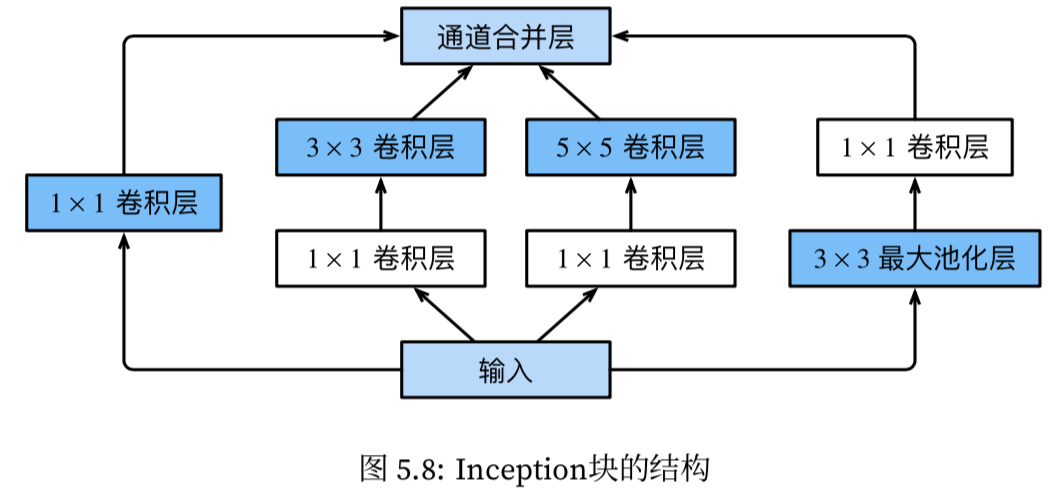
\includegraphics[width=0.6\textwidth]{note_images/inception_block.png} %插入图片,[]中设置图片大小,{}中是图片文件名
  \end{figure}

  \quad inception块结构表示:($n_1$, ($n_{21}$, $n_{22}$), ($n_{31}$, $n_{32}$), $n_4$) 
  
  \quad \quad 第一线路使用$n_1$通道
 
  \quad \quad 第二线路第一卷积层使用$n_{21}$通道,第二层卷积层使用$n_{22}$通道 1填充
 
  \quad \quad 第三线路第一卷积层使用$n_{31}$通道,第二层卷积层使用$n_{32}$通道 2填充
  
  \quad \quad 第四线路第一最大池化层使用(3, 3)窗口 1填充,第二层卷积层使用$n_4$通道

  \quad 每一卷积层都使用relu激活函数

  \quad 所有层输出作为不同通道结果,即最终有$n_1 + n_{22} + n_{32} + n_4$通道

  GoogLeNet结构:

  \quad 5个串联模块,每一卷积层使用relu激活函数,每一模块间使用 (3, 3)窗口\ 步幅2\ 1填充\ 池化层

  \quad 1. 64通道(7, 7)kernel 2步幅\ 3填充卷积层 + 模块间池化层

  \quad 2. 64通道(1, 1)kernel卷积层 + 64 * 3通道(3, 3)kernel 1填充卷积层 + 模块间池化层

  \quad 3. 串联2 inception 块 + 模块间池化层,分别有结构

  \quad \quad (64, (96, 128), (16, 32), 32),通道比\texttt{2:4:1:1}

  \quad \quad (128, (128, 192), (32, 96), 64),通道比\texttt{4:6:3:2}

  \quad 4. 串联5 inception 块 + 模块间池化层,

  \quad \quad (192, (96, 208), (16, 48), 64)

  \quad \quad (160, (112, 224), (24, 64), 64)

  \quad \quad (128, (128, 256), (24, 64), 64)

  \quad \quad (112, (144, 288), (32, 64), 64)

  \quad \quad (256, (160, 320), (32, 128), 128)

  \quad 5. 串联2 inception 块 + 全局平均池化层

  \quad \quad (256, (160, 320), (32, 128), 128)

  \quad \quad (384, (192, 384), (48, 128), 128)

  \quad 6. 全连接层,节点数和分类类别数相同

% --------------------------------------------------------------------------
% |                            CNN优化方法                                  |
% --------------------------------------------------------------------------
\section{CNN优化方法}
\noindent \textbf{批量归一化 batch normalization}

  \textbf{1. 对全连接层做批量归一}

  \quad 处于\ 输入的仿射变换\ 和\ 激活函数间,即\ 输出 = $\phi (BN(x))$ $BN$为批量归一计算

  \quad 1. 对于批量仿射 $x = Wu + b$,求标准化$\hat{x}_i = \frac{{x_i} - \mu}{\sqrt{\sigma^2 + \varepsilon }}$。$\mu $和 $\sigma$都为此组仿射变换的结果

  \quad 2. $BN(x) = \gamma * \hat{x}_i + \beta $,$\gamma$拉伸 $\beta$偏移。* + 为按元素加法 乘法

  \textbf{2. 对卷积层做批量归一}

  \quad 处于\ 卷积计算\ 和\ 激活函数\ 间,卷积计算 + 批量归一 + 激活函数 + 池化层

  \quad 各通道独立计算,各有独立拉伸$\gamma$ 偏移$\beta$。
  
  \quad $\sigma$, $\mu$为此通道\ 一批量内\ 所有通道\ 的所有元素\ 的总体方差,平均值

  \quad 得到$\sigma$, $\mu$后对此通道此批量内所有元素求标准化

  \quad 最终对此通道\ 
  \ 偏移\\
\textbf{ResNet残差网络}

  \textbf{残差块}

  \quad 训练时期望输出为f(x) - x,而非直接使用f(x)期望输出。得到f(x) - x后+x得到f(x)

  \quad 1. 卷积层(批量归一) + relu + 卷积层(批量归一) 得到$f(x) - x$
  
  \quad 2. [$f(x) - x$] + [(1, 1)卷积层对(x)卷积结果] + relu激活函数
  
  \quad \quad 第一卷积层:(3, 3)kernel 1填充 (通道数\ 步幅自定义)

  \quad \quad \quad 第234组残差组 第一残差块\ 第一卷积层步幅为2,否则为1

  \quad \quad 第二卷积层:(3, 3)kernel 1填充 1步幅 (通道数自定义)

  \quad \quad +x步骤的(1, 1)卷积层:(通道数\ 步幅自定义) 

  \quad \quad \quad 第234组残差组\ 第一残差块使用(1, 1)卷积层,步幅为2,否则直接+x

  \quad \quad 3层卷积层通道数共享同一自定义值,\textbf{要求2层卷积层输入输出通道数一致}

  ResNet-18模型:共18卷积层

  \quad 1. 64通道(7, 7)kernel 2步幅 3填充\ 批量归一卷积层 + (3, 3)窗口 2步幅 1填充最大池化层

  \quad 2. 4组\ 残差块,每组包含多个残差块

  \quad \quad 第一组 2个残差块\ 输出通道数和1中输出通道数一致
  
  \quad \quad 第二三四组\ 各2个残差块\ 输出通道数为前一层通道数$*2$

  \quad 3. 全局平均池化层 + 对应输出结果数全连接层\\
\textbf{DenseNet稠密连接网络}

  类似ResNet残差网络,+x步变为concat x连在输出结果后,即x直接传向下一层

  \textbf{稠密块}

  \quad 多组(批量归一 + relu + (3, 3)kernel 1填充卷积层 + concat x) 卷积层通道数相同

  \quad concat操作为在通道纬度的concat,即输入x作为额外输出通道。

  \quad 增长率 = 输出通道 - 输入通道 = 卷积层通道数

  \textbf{过渡层}

  \quad 批量归一 + relu + (1, 1)卷积层 + (2, 2)窗口 2步幅平均池化层
  
  \quad 使用(1, 1)卷积层减小通道数,2步幅平均池化层减小矩阵大小

  \quad \quad 卷积层通道数 = 输出通道数 / 2

  DenseNet模型

  \quad 1. 64通道(7, 7)kernel 2步幅 3填充\ 批量归一卷积层 + (3, 3)窗口 2步幅 1填充最大池化层

  \quad 2. 4组稠密块,由3个过渡层分隔

  \quad \quad 4层稠密块卷积层数可以不相同

  \quad 3. 批量归一 + relu + 全局平均池化层 + 对应输出结果数全连接层

% --------------------------------------------------------------------------
% |                             循环神经网络                                 |
% --------------------------------------------------------------------------
\section{RNN循环神经网络}

\noindent 记录数据状态,根据以往状态和当前输入决定输出\\
\textbf{n阶马尔科夫链}:一个词的出现仅和前n个词有关\\
\textbf{语言模型}:词序($w_1$, $w_2$, ..., $w_T$)的出现可能性为

  $P(w_1, w_2,...,w_T)\approx \prod_{t=1}^{T} P(w_t|w_{t-(n-1)},...,w_{t-1})$

  称n元语法,每一$w_t$为一时间步中出现的词\\
\textbf{处理语言模型}:将每一文字转化为索引,使用索引做训练参数集\\
\textbf{one\_hot表示}:索引为$i$的词对应one\_hot向量$[v_0 = 0, v_1 = 0, ..., v_i = 1, v_{i+1} = 0, ...]$\\
\textbf{采样方式}:

  $BATCH\_SIZE$ 每次采集的样本数
  
  $NUM\_STEPS$ 每个样本包含的时间步数,

  \textbf{1 随机采样}:

  \quad [1 2 3 4] [5 6 7 8] [9 10 11 12] [13 14 15 16]

  \quad 将所有样本分为头尾相连的组,每组有相等可能性被取值,每次随机取BATCH\_NUM组

  \quad 训练来自不同批量的样本时不能将前一次隐藏层结果纳入计算
  
  \textbf{2 相邻取样}:

  \quad [1 2 3 4    ] [5 6 7 8    ] [9 10 11 12 ] [13 14 15 16]

  \quad [17 18 19 20] [21 22 23 24] [25 26 27 28] [29 30 31 32]

  \quad 将样本填入BATCH\_NUM行矩阵,再分为(BATCH\_NUM, NUM\_STEPS)的小矩阵,每次每个小矩阵有等可能性被选择
  
  \quad 仅需在训练一开始初始化隐藏层结果,而非在每一批量开始初始化\\
\textbf{裁剪梯度}

  将所有参数拼接成向量$g$,进行裁剪:$g' = min(\frac{\theta}{||g||}, 1)g$\\
\textbf{困惑度}

  = exp(交叉熵损失函数值)\\
\textbf{RNN实现}

  模型:

  \quad 1.隐藏层$H_t = \phi(X_tW_{xh} + H_{t-1}W_{hh} + b_h)$

  \quad \quad $X_t$为上一时间步的词

  \quad \quad $H_{t-1}$项为隐藏层前一次输出,第一个时间步使用全零$H_{t-1}$矩阵

  \quad 2.输出层$O = HW_{hq} + b_q$
  
  实现:
  
  \quad 输入:(批量大小, 时间步数) 每一元素为词的编号
  
  \quad \quad 输入转换为\ 时间步数 * (批量大小, 词典大小) 个矩阵,第$i$矩阵第$j$行对应\ 批量中第$j$样本\ 第$i$时间步的词的one\_hot向量
  
  \quad 激活函数使用$tanh$
  
  \quad 计算:

  \quad \quad $H_t = \phi(X_tW_{xh} + H_{t-1}W_{hh} + b_h)$

  \quad \quad $O = HW_{hq} + b_q$
  
  \quad \quad 遍历前多个时间步的(批量大小, 词典大小)矩阵,每一时间步矩阵即$X_t$。
  
  \quad \quad 训练时输入一段时间步$[w_{t0}, w_{t1}]$,输出即为预测$[w_{t0+1}, w_{t1+1}]$的词
  
  \quad \quad \quad \textbf{1.输出的词在$[w_{t0+1}, w_{t1}]$时间步不一定和训练集一致}

  \quad \quad \quad \textbf{2.输出为$(t1+1) - (t0+1)$个时间步的预测词,每个词使用one\_hot向量表示}
  
  \quad \quad 代价函数使用 $(t1+1) - (t0+1)$个时间步one\_hot表示\ 和\ 每一$[w_{t0+1}, w_{t1}]$时间内词的one\_hot表示\ 的交叉熵\\
\textbf{通过时间反向传播}

  \textbf{有关时间步的损失函数}:$L = \frac{1}{T}\sum_{t = 1}^{T} l(o_t, y_t) $

  \textbf{** 反向传播公式 **}\\\\
\textbf{GRU 门控循环单元}

  替代原计算隐藏状态方法,应对梯度衰减
  \begin{figure}[H] %H为当前位置,!htb为忽略美学标准,htbp为浮动图形
    \centering %图片居中
    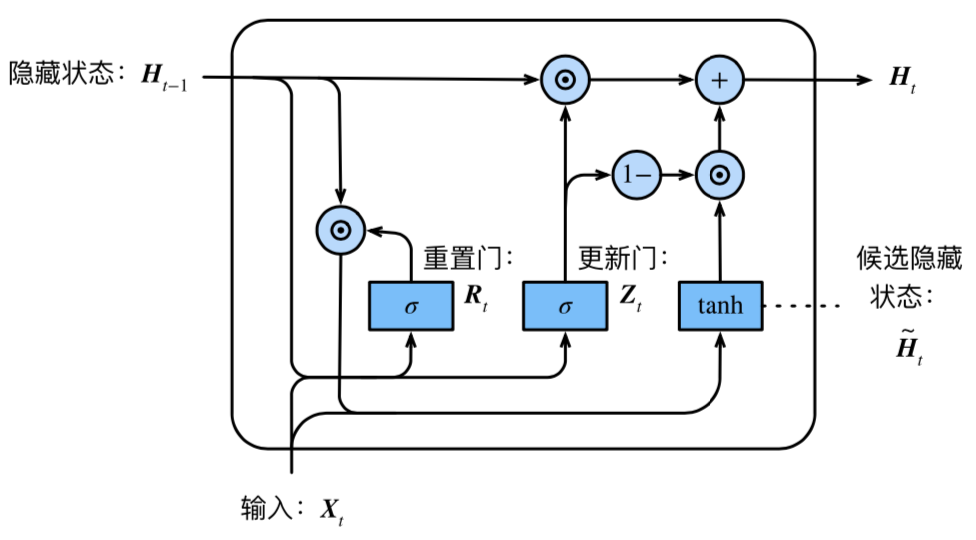
\includegraphics[width=0.6\textwidth]{note_images/GRU.png} %插入图片,[]中设置图片大小,{}中是图片文件名
  \end{figure}

  \textbf{reset gate重置门 update gate更新门}:

  \quad 得到上一层影藏层结果$H_{t-1}$ 当前时间步输入$X_t$

  \quad 隐藏层$R_t = \sigma(X_tW_{xr} + H_{t-1}W_{hr} + b_r)$
  
  \quad 更新层$Z_t = \sigma(X_tW_{xz} + H_{t-1}W_{hz} + b_z)$

  \quad \quad W 为权重参数\ b为偏差参数 $\sigma$为sigmoid函数

  \textbf{候选隐藏状态}

  \quad 候选隐藏状态$\tilde{H_t} = tanh(X_tW_{xh} + (R_t \odot  H_{t-1})W_{hh} + b_h)$

  \quad \quad $\odot$为按元素相乘,使得重置门中对应位置值为0的元素被丢弃

  \textbf{隐藏状态}

  \quad $H_t = Z_t \odot H_{t-1} + (1-Z_t)\odot \tilde{H_t}$\\
\textbf{LSTM长短期记忆 门控循环网络}
  \begin{figure}[H] %H为当前位置,!htb为忽略美学标准,htbp为浮动图形
    \centering %图片居中
    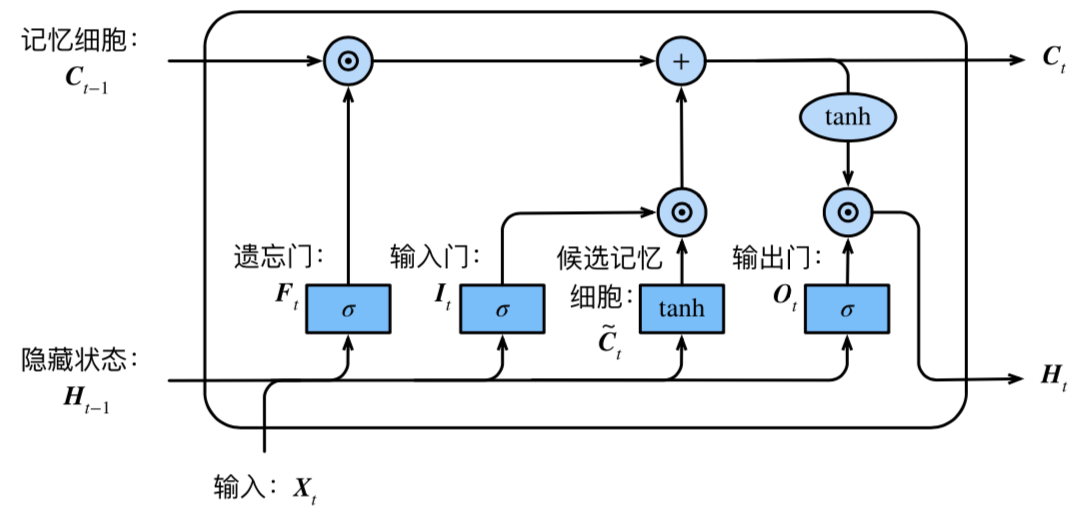
\includegraphics[width=0.6\textwidth]{note_images/LSTM.png} %插入图片,[]中设置图片大小,{}中是图片文件名
  \end{figure}
\textbf{深度循环神经网络}

  包含多个隐藏层的RNN
  \begin{figure}[H] %H为当前位置,!htb为忽略美学标准,htbp为浮动图形
    \centering %图片居中
    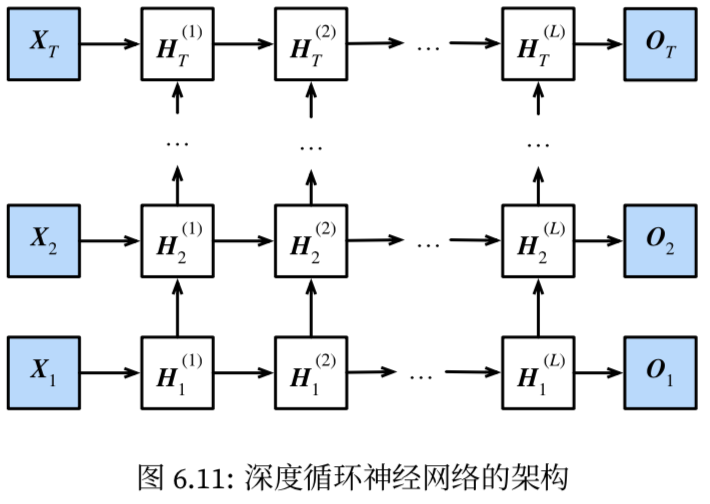
\includegraphics[width=0.6\textwidth]{note_images/deep_RNN.png} %插入图片,[]中设置图片大小,{}中是图片文件名
  \end{figure}
  结构:

  \quad 隐藏层\textbf{输出}为$H_i^{(1)} \space H_i^{(2)}...H_i^{(n)}$,第$i$次forward对应图中一行,即$X_i \rightarrow  H_i^{(1)} \rightarrow  ... \rightarrow  H_i^{(n)} \rightarrow O_i$

  \quad 第$i$次计算中:

  \quad \quad $l = 1$ 隐藏层输出 $H_i^{(1)} = \phi (X_iW_{xh}^{(1)} + H_{i-1}^{(l)}W_{hh}^{(1)} + b_h^{(1)})$

  \quad \quad \quad 和单层隐藏层RNN的\ 隐藏层输出公式\ 一致

  \quad \quad $l = 2,3...n$ 隐藏层输出 $H_i^{(l)} = \phi (H_i^{(l-1)}W_{xh}^{(l)} + H_{i-1}^{(l)}W_{hh}^{(l)} + b_h^{(l)})$

  \quad \quad \quad 即$l=1$公式中将输入变为前一隐藏层输出

  \quad \quad 输出层 $O_i = H_{i}^{(n)}W_{hq} + b_q$\\
\textbf{双向循环神经网络}

  允许神经网络根据前后的词序决定当前时间步的词
  \begin{figure}[H] %H为当前位置,!htb为忽略美学标准,htbp为浮动图形
    \centering %图片居中
    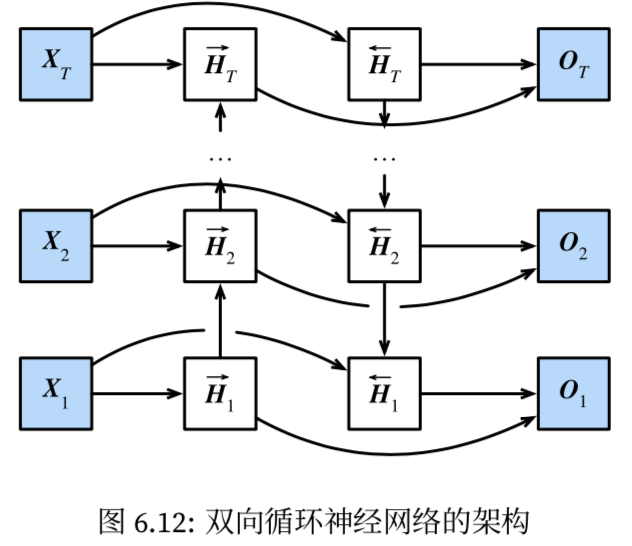
\includegraphics[width=0.6\textwidth]{note_images/double_deep_RNN.png} %插入图片,[]中设置图片大小,{}中是图片文件名
  \end{figure}
  结构:

  \quad 仅有2隐藏层,分为\ 正向隐藏层\ 反向隐藏层,分别输出$H^{(f)}$ $H^{(b)}$

  \quad 第$i$次计算中

  \quad \quad $H_i^{(f)} = \phi (X_iW_{xq}^{(f)} + H_{i-1}^{(f)}W_{hh}^{(f)} + b_h^{(f)})$

  \quad \quad $H_i^{(b)} = \phi (X_iW_{xq}^{(b)} + H_{i+1}^{(b)}W_{hh}^{(b)} + b_h^{(b)})$

  \quad \quad $O_i = H_iW_{hq} + b_q$

  \quad \quad \quad $H_i = (H_i^{(f)}, H_i^{(b)})$,为正向\ 反向隐藏层的输出concat


% --------------------------------------------------------------------------
% |                             代码算法优化                                 |
% --------------------------------------------------------------------------
\section{代码算法优化}
\noindent \textbf{Stochastic Gradient Decent 随机梯度下降}:采样方法

  每次迭代随机选择一个\textbf{样本},得到权重针对此样本的斜率进行梯度下降\ 而不是求参数针对所有样本的代价函数斜率。开销从O(n)变为O(1)

  \quad 即 任取的样本j,SGD迭代为$\theta_i = \theta_i - \eta \frac{d J^{(j)}(\theta)}{d \theta_i}$\\
\textbf{batch gradient descent 小批量随机梯度下降}:采样方法

  每次迭代随机选择一组样本 $B$,计算参数关于$B$的代价函数斜率

  重复采样:允许$B$中重复出现同一样本。反之不重复采样

  随迭代次数增加,学习率可减小,使学习率和斜率的乘积方差减小\\\\
\textbf{动量法}:迭代方法

  解决固定一学习率值无法同时满足多个参数的学习率范围,导致某些参数发生学习太慢,某些参数不断越过最优解

  定义:
  
  \quad 向量$v_t$为第t次迭代每一参数的速度变量

  \quad 向量$x_t$为第t次迭代参数向量

  \quad 向量$g_t$为第t次迭代每一参数的斜率

  迭代:

  \quad $v_t = \gamma v_{t-1} + \eta_t g_t$

  \quad $x_t = x_{t-1} - v_t$\\
\textbf{AdaGrad算法}:迭代方法

  根据参数斜率调整学习率

  定义向量$s_t$为第t次迭代累加变量,累计每一参数的斜率平方和

  迭代:

  \quad $s_t = s_{t-1} + g_t \odot g_t$

  \quad $x_t = x_{t-1} - \frac{\eta}{\sqrt{s_t + \epsilon } } \odot g_t$

  \quad \quad 即每一参数有变量记录所有斜率历史,每次迭代时\ 学习率/斜率历史l2 norm

  由于累加变量斜率历史,学习率始终降低,造成学习缓慢\\
\textbf{RMSProp 算法}:迭代方法

  解决AdaGrad末期学习率过低问题

  迭代:
  
  \quad $s_t = \gamma s_{t-1} + (1-\gamma)g_t \odot g_t$即 对$s_t$按元素平方做指数加权

  \quad $x_t$同AdaGrad算法\\
\textbf{AdaDelta 算法}:迭代方法

  解决AdaGrad末期学习率过低问题,不使用超参数

  定义:

  \quad 向量$g_t'$记录参数变化量

  \quad 向量$\varDelta x_t$对$g_t'$按平方做指数加权

  迭代:

  \quad $s_t = \gamma s_{t-1} + (1-\gamma)g_t \odot g_t$\ \ \ \ 同RMSProp

  \quad $\varDelta x_t = \gamma \varDelta x_{t-1} + (1-p)g_t' \odot g_t'$\ \ \ \ $\varDelta x_t$初始化为全零向量

  \quad $g_t' = \sqrt{\frac{\varDelta x_t + \epsilon }{s_t + \epsilon }} \odot g_t $

  \quad $x_t = x_{t-1} - g_t'$\ \ \ \ \ \ \ \ \ \ $g_t'$即参数变化率\\
\textbf{Adam 算法}:迭代方法

  定义:

  \quad $v_t$ t时间步的\ 动量变量

  \quad $s_t$ t时间步的\ 指数加权移动平均

  \quad $g_t$ t时间步\ 小批量\textbf{随机梯度}

  \quad $0\leq \beta_1<1$所有\ 动量变量的权重超参数。常取$0.9$
  
  \quad $1\leq \beta_2<1$ 所有\ 指数加权移动平均变量超参数。常取$0.999$

  迭代:

  \quad $v_t = \beta_1v_{t-1} + (1 -\beta_1)g_t$

  \quad $s_t = \beta_2 s_{t-1} + (1-\beta_2)g_t \odot g_t$

  \quad $\hat{v}_t = \frac{v_t}{1-\beta_1^t}$

  \quad $\hat{s}_t = \frac{s_t}{1-\beta_2^t}$

  \quad \quad 使用$\hat{v}_t$, $\hat{s}_t$\textbf{偏差修正}
  
  \quad \quad \quad 使得每一时间步t前的权重和为1,使得在时间步数较小时动量值不受权重影响

  \quad \quad \quad \quad 例:不使用偏差修正:$v_1 = 0.1g_1$

  \quad $g_t' = \frac{\eta \hat{v}_t}{\sqrt{\hat{s}^t} + \epsilon}$

  \quad \quad $\epsilon $常取$10^{-8}$

  \quad $x_t = x_{t-1} - g_t'$


% --------------------------------------------------------------------------
% |                              计算机视觉                                  |
% --------------------------------------------------------------------------
\section{计算机视觉}
\noindent 提升模型泛化能力方法:图像增广\ 图像微调\\
\textbf{图像增广}

  对图像随机变换,产生相似样本。扩大训练集

  方法:

  \quad 翻转:有固定几率上下/左右翻转

  \quad 裁剪:随机裁剪原图10\%-100\%面积的图像,宽高比0.5-2,并拉伸至固定像素大小

  \quad 变化颜色:调整亮度\ 色调\ 对比度\ 饱和度\\
\textbf{微调}

  假设:

  \quad 源模型包含的知识和目标模型紧密相连
  
  \quad 源模型输出层不能直接用于目标模型

  \quad 目标数据集远小于源数据集

  方法:
 
  \quad 1. 在源数据集上训练一神经网络,称源模型

  \quad 2. 创建一新神经网络,称目标模型,复制源模型除了输出层的所有结构和参数

  \quad 3. 为目标模型添加输出层,节点数对应输出种类,随机初始化模型参数

  \quad 4. 在目标数据集上训练目标模型,微调hidden layer参数,从头训练输出层参数

  \quad \quad 通过提高输出层学习率,降低隐藏层学习率达到重新训练输出层,微调隐藏层的目的。学习率相差可达1000倍\\
\textbf{目标检测}

  锚框:标记一个物体的范围框

  交并比IoU:两锚框\ 相交面积/相并面积

  训练集:每一锚框有对应的目标的标签\ 相对目标范围框的偏移

  \quad 赋目标框

  \quad \quad 1. 对锚框组$A_1, A_2, ...A_n$,目标框组$B_1, B_2, ...B_m$定义矩阵X,

  \quad \quad \quad X为(n, m),包含每一锚框相对每一目标框的交并比

  \quad \quad 2. 找到X中值最大项$x_{ij}$,则$A_i$对应目标$B_j$,移除X中$i$行$j$列

  \quad \quad 3. 重复找到剩余矩阵中的最大项并移除,最终有$m$锚框对应目标,剩余$n-m$锚框

  \quad \quad 4. 对每一未对应锚框$A_i$,寻找X中i行最大交并比,若值大于阈值,为$A_i$分配对应目标框,若没有交并比大于阈值,目标框为整个图片。

  \quad \quad 被赋予目标框的锚框称正类锚框,否则为负类锚框

  \quad 赋偏移量

  \quad \quad 对锚框$A_i$有$(x_a, y_a, h_a, w_a)$,对应目标框$B_j$有$(x_b, y_b, h_b, w_b)$

  \quad \quad 设置常数$\mu_x = \mu_y = \mu_w = \mu_h = 0$, $\sigma_x = \sigma_y = 0.1$, $\sigma_w = \sigma_h = 0.2$

  \quad \quad 偏移量为$(\frac{\frac{x_b - x_a}{w_a} - \mu_x}{\sigma_x},\frac{\frac{y_b - y_a}{h_a} - \mu_y}{\sigma_y}, \frac{log(\frac{w_b}{w_a}) - \mu_w}{\sigma_w}, \frac{log(\frac{h_b}{h_a}) - \mu_h}{\sigma_h})$

  非极大值抑制:non-maximum suppression

  \quad 在显示结果阶段,去除重复对一个物体分类的锚框

  \quad 锚框置信度:一个锚框$A_i$针对所有目标锚框$B$计算概率,$A_i$最大概率符合的目标锚框对应$A_i$的预测类别,此最大概率为$p$。概率不是锚框和目标锚框的交并比,而是输出层输出的\ 每一锚框与每一类别\ 的可能性

  \quad 算法:

  \quad \quad 1. 计算每一锚框置信度,选取最高的锚框$A_i$

  \quad \quad 2. 将所有和$A_i$交并比高于阈值的锚框删除

  \quad \quad 重复1.2.步,直至没有锚框剩余

  多尺度目标检测:仅适用部分像素点作为锚框的中心,减少锚框数量,减少计算\\\\
\textbf{SSD 单发多框检测}

  \begin{figure}[H] %H为当前位置,!htb为忽略美学标准,htbp为浮动图形
    \centering %图片居中
    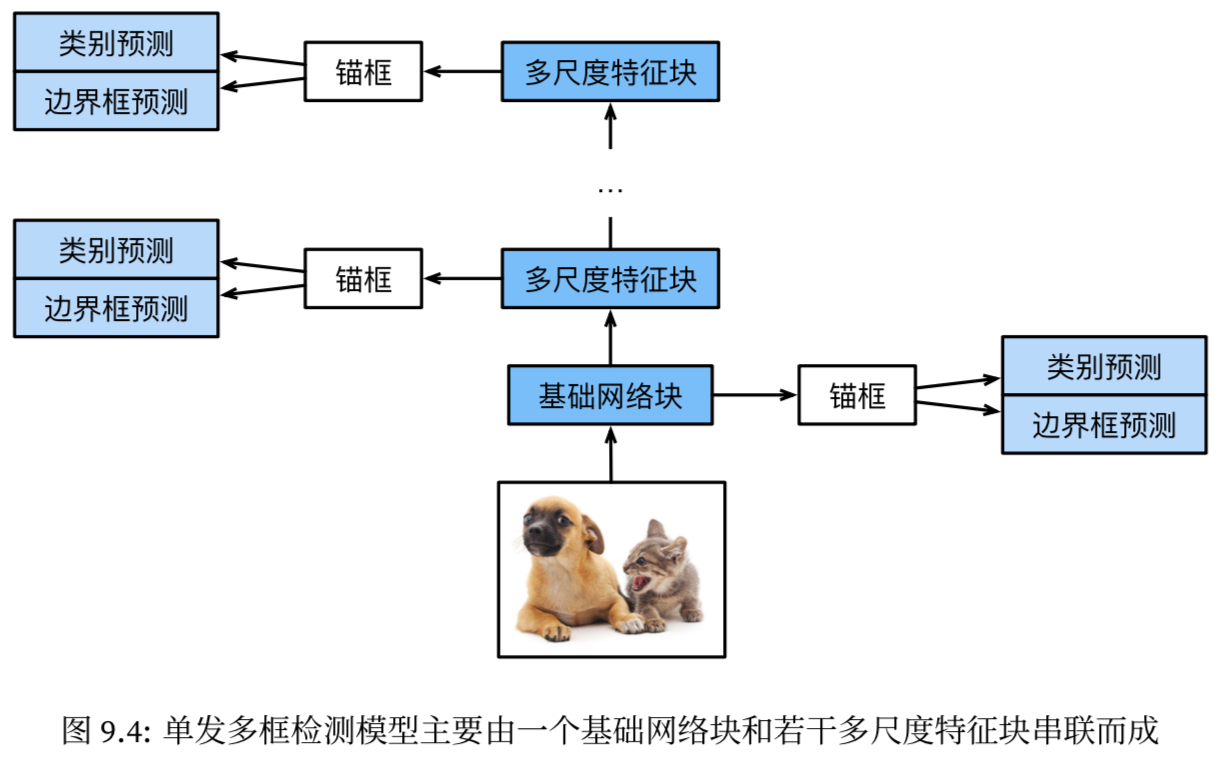
\includegraphics[width=0.6\textwidth]{note_images/SSD_archi.png} %插入图片,[]中设置图片大小,{}中是图片文件名
  \end{figure}

  \textbf{类别预测层}:

  \quad 对锚框只进行分类,不进行偏差计算。
  
  \quad 假设锚框中心像素有(h, w)个,每个中心点生成a个锚框,每个锚框需匹配进$(q+1)$个分类,多1分类对应负类分类

  \quad \quad 将锚框看做多层,每层$h*w$个,共$a$层,层编号为$c_1, c_2, ..., c_a$

  \quad 方法0:对每一锚框使用全连接层分类,即每一像素输入全连接网络,最终有匹配类别个数的输出层,判断锚框分类

  \quad \quad 造成参数过多,无法训练

  \quad 方法1:使用卷积层通道数输出类别

  \quad \quad 包含一个保持输入高\ 宽的卷积层,如\ 1填充 (3, 3)kernel的卷积层

  \quad \quad 输出通道数为$a * (q+1)$,每一通道输出仍为矩阵,第$(i-1)*(q+1) + j$通道包含锚框层$c_i$中所有锚框对分类j的匹配可能性

  \textbf{边界框预测层}:

  \quad 输入结构同类别预测层,输出通道数为$a * 4$,4对应一个锚框有4个偏差值,每一通道输出仍为矩阵,第$(i-1)*(q+1) + j$通道包含锚框层$c_i$中所有锚框的第$i$号偏差值

  \textbf{连接多尺度预测}:

  \quad 将不同多尺度特征块和基础网络块产生的\ 类别\ 边界预测层结果\ 合并
  
  \quad (批量大小, 通道数, 高, 宽)\ 转为 (批量大小, 通道数 * 高 * 宽)
  
  \textbf{高宽减半块}:

  \quad 1.两组[(3, 3)kernel 1填充\ 卷积层 + 批量归一化 + relu]
  
  \quad 2.(2, 2)窗口\ 2步幅\ 最大池化层

  \textbf{基础网络块}

  串联3块高宽减半块,分别有16, 32, 64通道

  \textbf{整体模型}
  
  \quad 结构对应图例,每一模块有\ 类别\ 边界预测层

  \quad 1. 基础网络块

  \quad 2-4. 高宽减半块 

  \quad 5. 仅包含全局最大池化层\ 高宽降至1

  \quad \textbf{得到输出集}

  \quad \quad 5层\ 类别\ 边界预测结果通过concat得到总体类别预测\ 边界预测,用于计算代价。类别预测使用\texttt{SoftmaxCrossEntropyLoss},边界预测使用\texttt{L1Loss}。\textbf{由于所有坐标通过百分比表示,可直接和标签集一一对应,不受卷积层对矩阵大小影响}

  \quad \quad \quad 即\ concat结果由多个 (4个百分比定义一锚框,类别预测值\ 边界预测值)

  \quad \textbf{得到标签集}

  \quad \quad 对于5层中所有使用过的锚框,使用\textbf{目标检测}章节的算法对每一锚框添加标签\ 偏移量。添加结束的训练集和输出集元素一一对应。\\
\textbf{R-CNN 区域卷积神经网络}

  对每一提议区域做卷积神经网络训练,耗时长\\
\textbf{Fast R-CNN}

  \begin{figure}[H] %H为当前位置,!htb为忽略美学标准,htbp为浮动图形
    \centering %图片居中
    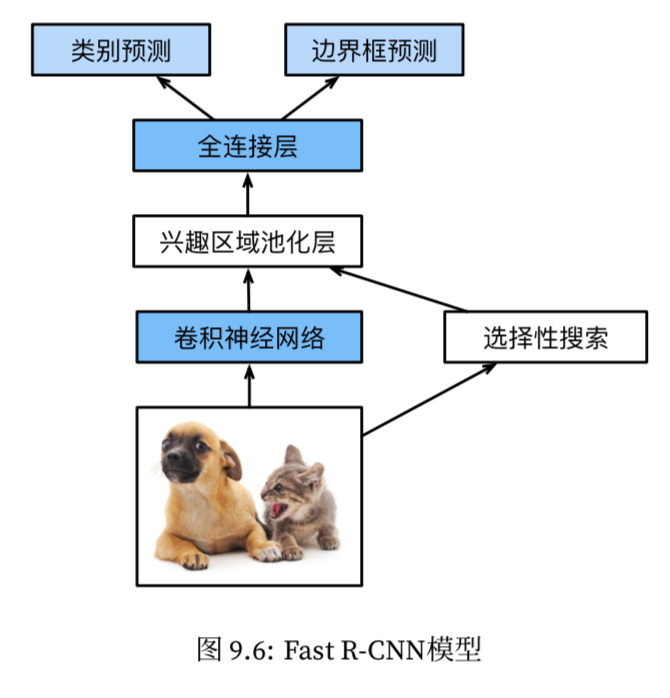
\includegraphics[width=0.6\textwidth]{note_images/Fast_R-CNN.png} %插入图片,[]中设置图片大小,{}中是图片文件名
  \end{figure}

  与\texttt{R-CNN}区别:

  \quad 1.提取特征的神经网络为整个图像

  \quad \quad 当输入为一张图片时,输出形状为$(1, c, h_1, w_1)$

  \quad 2.选择性搜索$n$个提议区域,

  \quad 3.兴趣区域池化层\ 输出$(n, c, h_2, w_2)$

  \quad \quad 可指定池化窗口任意矩形区域作为一个池化结果的源,所以可产生任意形状池化结果

  \quad \quad 例:
    $\begin{bmatrix}
      x_{11} & x_{12} & x_{13} \\
      x_{21} & x_{22} & x_{23} \\
      x_{31} & x_{32} & x_{33}
      \end{bmatrix}$
    可取$\begin{bmatrix}
      x_{11} & x_{12} \\
      x_{21} & x_{22} 
      \end{bmatrix}$
    和$\begin{bmatrix}
      x_{31} & x_{32}
      \end{bmatrix}$
    做输出$y_{11}$和$y_{21}$的来源

  \quad 4.全连接层\ 输出变为$(n, d)$,$d$为超参数

  \quad 5.预测类型使用$softmax回归$,输出$(n, q)$

  \quad \quad 预测边界框时,输出$(n, 4)$\\
\textbf{图像分割}

  区分图片中一个物体的不同部分,不将每一物体和标签对应\\
\textbf{实例分割}

  区分一个像素属于哪一物体,即使两物体为同一标签下的实例\\
\textbf{semantic segmentation语义分割}

  图像预处理:不使用拉伸,仅适用随机图片裁剪,裁剪得到图片一块固定形状的小图,作为训练集

  \textbf{FCN 全卷积网络}

  \quad 结构:
  
  \quad \quad 1.使用卷积神经网络\ 抽取图像特征

  \quad \quad 2.(1, 1)卷积层\ 通道数变为类别个数

  \quad \quad 3.转置卷积层\ 将图像的高宽变为输入图像的尺寸,作用仅为将2.中的图片分类反卷积得到图片表示,所以输入通道数 = 输出通道数 = 类别个数

  \quad 例:

  \quad \quad 1.ResNet-18预先训练神经网络抽取图像特征\ 丢弃最后全局平均池化层+全连接层

  \quad \quad 2.(1, 1)卷积层,通道数 = 类别数$n$
  
  \quad \quad 3.转置卷积层将(1, 1)卷积层每一通道的输出转换回图片大小的矩阵,每一元素为类别对应像素的index

  \quad 输出图片:
  
  \quad \quad 1.对一个图片的$n$个通道中结果\ 合并为唯一矩阵,新矩阵每一元素 = $n$个矩阵中对应位置最大值

  \quad \quad \quad 即\ 输出的$n$个矩阵代表图像符合每一类别的区域,对一个位置的元素取最大值即判断此位置最优先属于哪一类别
  
  \quad \quad 2.替换1.中输出的矩阵元素,每一元素替换为此位置的RGB向量\\
\textbf{样式迁移}

  \begin{figure}[H] %H为当前位置,!htb为忽略美学标准,htbp为浮动图形
    \centering %图片居中
    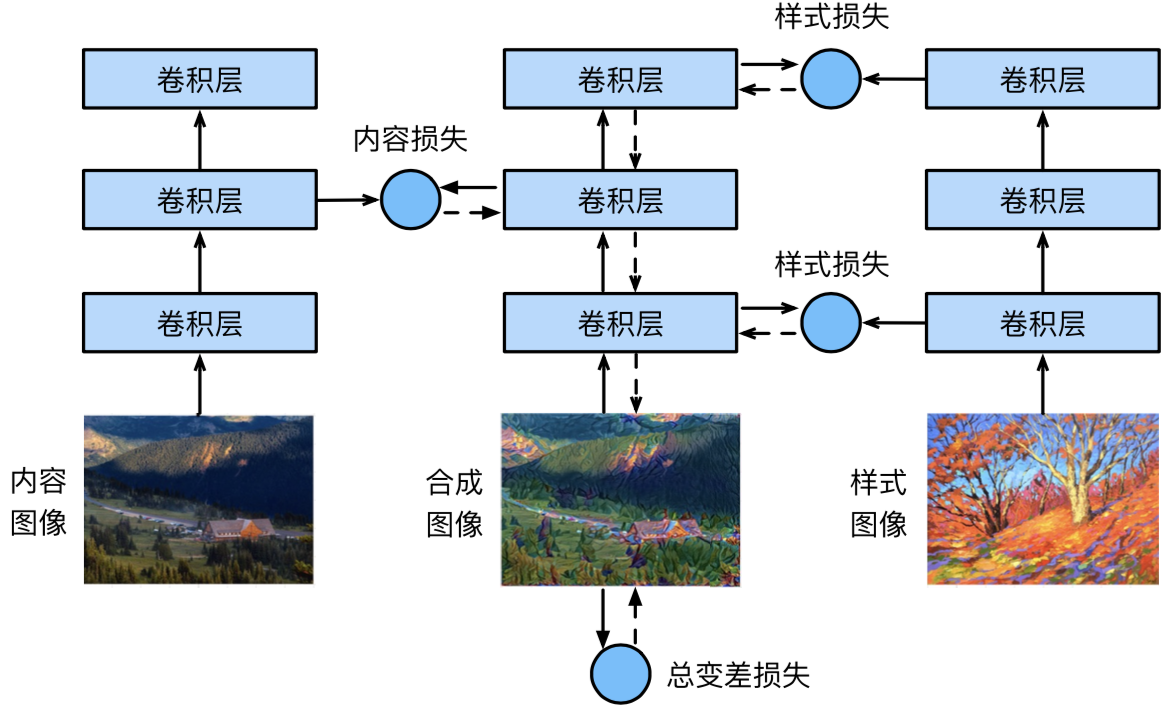
\includegraphics[width=0.6\textwidth]{note_images/style-transfer.png} %插入图片,[]中设置图片大小,{}中是图片文件名
  \end{figure}

  得到\ 内容图像\ 样式图像,输出合成图像

  \textbf{图像预处理}:将输入图片在RGB\ 3通道内分别做标准化

  \textbf{图像后处理}:将输出矩阵标准化的值\ 转回\ 像素值

  \textbf{抽取特征}:

  \quad 使用VGG-19预训练参数抽取图像特征

  \quad \quad 选择VGG靠近输出的层,称内容层,避免保留过多内容图像的细节

  \quad \quad 选择多个中间层的输出匹配样式,称样式层

  \textbf{损失函数}

  \quad 损失函数为内容\ 样式\ 总变差损失函数的加权和

  \quad \textbf{内容损失函数}:

  \quad \quad 使用平方代价函数,计算\ 合成图像\ 和\ 内容图像\ 在\ 内容特征上的误差

  \quad \quad 输入张量为\ 内容图像和合成图像\ 通过抽取特征后内容层的输出

  \quad \textbf{样式损失函数}:

  \quad \quad 输入张量为样式层输入

  \quad \quad 对每一样式层:

  \quad \quad \quad 1.将$c$通道$(h, w)$的样式层输出转为$(c, hw)$的矩阵$X$

  \quad \quad \quad 2.计算$X$的Gram matrix, $XX^T$。元素$(XX^T)_{ij}$即$x_i \cdot x_j$,代表通道i和j的相关性

  \quad \quad \quad 3.传入内容图像\ 合成图像,对每一样式层输出做平方代价函数

  \quad \textbf{总变差损失}:

  \quad \quad 输入仅为合成图像,对合成图像使用总变差降噪

  \quad \quad $J = \sum_{i, j} |x_{i,j} - x_{i+1,j}| + |x_{i,j} - x_{i,j+1}|$

  \quad \quad \quad 即\ 对每一合成图片的像素,求其和右方\ 下方像素的差值。最后求和

  \textbf{样式迁移模型}:

  \quad 使用每一VGG块的第一卷积层做样式层,第四卷积块的最后一卷积层做内容层

% --------------------------------------------------------------------------
% |                             自然语言识别                                 |
% --------------------------------------------------------------------------
\section{自然语言识别}
\noindent \textbf{一. 词嵌入}:将词和实数向量对应,词间夹角$\frac{x^Ty}{||x||\space||y||} \in [-1, 1]$为词的相似度\\
定义:

  $S$:词序集合,包含多个词序,包含重复的词

  $\mathcal{V} $:所有词的索引集合,即$nub(S)$

  $w_i$:一个词,索引为$i$

  $v_i$:词$w_i$对应的实数向量
  
  \quad 向量夹角余弦值$\frac{x^Ty}{||x||\space ||y||}$代表两个词的关联程度

  背景窗口大小$n$:定义对一个中心词$w_i$,背景词取值范围$=[$中心词$-n$, 中心词$+n]$。
  
  \quad 范围为词序内位置关系,不是索引序号关系。背景词和中心词必须在同一词序内

  \quad 当中心词一侧背景词个数$l<n$,填充$n-l$个无效词,随后由掩码舍弃不进入代价函数计算。

  给定中心词$w_c$,有单个背景词$w_o$的概率$P(w_o | w_c) = \frac{exp(u_o^Tv_c)}{\sum_{i\in\mathcal{V} } exp(u_i^Tv_c)}$\\
\textbf{跳字模型}:
  
  基于一个\textbf{中心词}生成才其周围的多个\textbf{背景词}

  \textbf{似然函数}:代表一段词序发生的可能性

  \quad 对中心词$w_c$,产生所有窗口内的背景词的概率为(假设背景词间$independent$)$P(c) = \prod_{c-n<j<c+n} P(w_j | w_c)$

  \quad (假设每一中心词产生背景词的可能性independent) 产生整个词序$S$的可能性:
  
  \quad \quad $P(S) = \prod_{0\leq c \leq |S|} P(c) = \prod_{c = 0}^{|S|-1} \prod_{j = c-n, j \neq c}^{c+n} P(w_j | w_c)$
  
  \textbf{代价函数}:基于似然函数,高似然代表低代价函数值

  \quad $J = -log(P(S)) = -\sum_{c = 0}^{|S|-1} \sum_{j = c-n, j \neq c}^{c+n} log(P(w_j | w_c))$

  \quad 求导: $\frac{d J}{d v_c} = -\sum_{c = 0}^{|S|-1} \sum_{j = c-n, j \neq c}^{c+n} \frac{d P(w_j | w_c)}{d v_c}$

  \quad \quad 对于每一中心词$v_c$有$\frac{d P(w_j | w_c)}{d v_c} = u_o^T - \sum_{j\in\mathcal{V}}P(w_j | w_c)u_j$\\
\textbf{连续词袋模型}

  与跳字模型不同处:中心词由背景词产生,和跳字模型相反

  给定背景词$W_o = w_{o_1}, w_{o_2}, ..., w_{o_{2m}}$,中心词$w_c$有出现概率:
  
  \quad $P(w_c | w_{o_1}, ..., w_{o_{2m}}) = \frac{exp(\frac{1}{2m}u_c^T(v_{o_1} + ... + v_{o_{2m}}))}{\sum_{i\in \mathcal{V} } exp(\frac{1}{2m}u_i^T(v_{o_1} + ... + v_{o_{2m}}))}$

  \quad \quad $= \frac{exp(u_c^T\bar{v}_o)}{\sum_{i\in \mathcal{V} } exp(u_i^T\bar{v}_o )}$

  \quad 1.使用\texttt{postierior estimate}计算得到,忽视$P(w_c)$项

  \quad 2.$\frac{1}{2m}$项为额外添加,使$\bar{v}_o = \frac{(v_{o_1} + ... + v_{o_{2m}})}{2m}$
  
  \textbf{似然函数}:

  \quad $\prod_{c \in \mathcal{V} } P(w_c | W_o)$

  \textbf{代价函数}:基于似然函数,高似然代表低代价函数值

  \quad $J = -log(\prod_{c \in \mathcal{V} } P(w_c | W_o))$

  \quad \quad $= -\sum_{c \in \mathcal{V} } (u_c^T\bar{v}_o - log(\sum_{i\in \mathcal{V} } exp(u_i^T\bar{v}_o )))$

  \quad 求导:$\frac{d J}{d v_{o_i}} = -\frac{1}{2m}(u_c - \sum_{j \in \mathcal{V} }P(w_j | W_o)u_j)$\\
\textbf{近似训练}:对跳字模型和词袋模型的优化

  避免每次梯度计算都包含词典大小的项数计算

  \textbf{负采样}

  \quad 定义:

  \quad \quad 背景词$w_o$出现在$w_c$背景窗的概率为$P(D = 1|w_c, w_o) = \sigma(u_c^Tv_o)$

  \quad \quad \quad $\sigma$为sigmoid激活函数,$D = 1$代表事件发生,$D = 0$代表未发生

  \quad 更改$P(w_o | w_c)$定义:$P(w_o | w_c) = P(D = 1| w_c, w_o)\prod_{k=1, w_k \in P(w)}^{K}P(D = 0 | w_c, w_k)$

  \quad \quad 根据$P(w)$分部取$K$个反样本,称噪声词,反样本不能为背景词

  \textbf{** 层序softmax **}\\
\textbf{二次采样}

  作用:对于一个词$w_0$,和低频词同时出现的情况\ 比\ 和高频词同时出现\ 对模型训练更加有用

  实现:
  
  \quad 数据集中每个词有$P(w_i) = max(1-\sqrt{\frac{t}{f(w_i)}}, 0)$几率被丢弃

  \quad \quad $f(w_i) = $ 出现$w_i$个数 / 总词数,即$w_i$出现频率

  \quad \quad $t$为超参数

  \quad 对每个$w \in S$,使用二次采样随机丢弃$w$,创建新的$S'$作为训练集\\
\textbf{word2vec词嵌入模型实现}

  目标:得到每一词的词向量,使有关联的词间向量夹角最小

  \textbf{嵌入层}

  \quad 得到词嵌入的层,输入词$w_i$索引$i$,输出权重矩阵第$i$行作为词向量

  \quad 嵌入层有权重矩阵,形状\texttt{(词典大小, 每个词向量纬度)}

  \textbf{前向计算}

  \quad 输入:中心词索引矩阵
    $\begin{bmatrix}
      [c_1] \\
      ... \\
      [c_b]
      \end{bmatrix}
    $+ (背景词, 噪声词)索引矩阵
    $\begin{bmatrix}
      [o_{11}, ..., o_{1n}, q_{11}, ..., q_{1k}] \\
      ... \\
      [o_{b1}, ..., o_{bn}, q_{b1}, ..., q_{bk}]
      \end{bmatrix}
    $

  \quad \quad $b$为批量大小

  \quad \quad $n$为窗口大小

  \quad \quad $k$为噪声词数量

  \quad \quad 两个输入矩阵元素皆为常数,非向量

  \quad 1.通过嵌入层变换为\ 中心词向量张量\texttt{(b, 向量长, 1)}
  $\begin{bmatrix}
    [u_{c_1}] \\
    ... \\
    [u_{c_b}]
    \end{bmatrix}
  $\ 背景噪声词向量张量\texttt{(b, 向量长, n+k)}
  $\begin{bmatrix}
    [v_{o_{11}}, ..., v_{o_{1n}}, v_{q_{11}}, ..., v_{q_{1k}}] \\
    ... \\
    [v_{o_{b1}}, ..., v_{o_{bn}}, v_{q_{b1}}, ..., v_{q_{bk}}]
    \end{bmatrix}
  $

  \quad 2.对两张量按行相乘,即得到\texttt{(b, 1, n+k)}张量
  $\begin{bmatrix}
    u_{c_1}^T * [o_{11}, ..., o_{1n}, q_{11}, ..., q_{1k}] \\
    ... \\
    u_{c_b}^T * [o_{b1}, ..., o_{bn}, q_{b1}, ..., q_{bk}]
    \end{bmatrix}
  $

  \quad 乘法为矩阵乘法,行向量$u_{c_1}^T$ 乘\ 矩阵$[o_{11}, ..., o_{1n}, q_{11}, ..., q_{1k}]$
  
  \quad 输出张量(b, 1, k+n),每一元素为背景词\ 噪声词和中心词的点乘,对应计算词向量夹角
  
  \textbf{代价函数}

  \quad 使用二元交叉熵函数,传入前向传播结果$P$,label$L$代表样本是否为正样本,掩码$M$代表样本是否有效

  \quad ** 如何联系可能性计算和夹角计算的关系\\
\textbf{fastText子词嵌入}:基于word2vec优化

  产生子词:在单词首尾添加\texttt{< >},取所有长度为$s$的子字符串 + 单词本身

  \quad 如,对单词\texttt{'where'}有子词\texttt{\{'<wh', 'whe', 'her', 'ere', 're>', '<where>'\}}

  每一子词都存在词典中,单个词对应的向量为子词向量和\\
\textbf{GloVe全局向量的词嵌入}:基于word2vec优化

  对每一中心词$w_i$,合并所有$w_i$的背景词,称多重集$\mathcal{C}_i$。多重集直接合并原集合,不删除重复项

  \quad 一个背景词$w_j$在$\mathcal{C}_i$中的出现次数称\ 重数,记做$x_{ij}$

  \quad 定义$x_i = |\mathcal{C}_i|$,为多重集集合大小

  \textbf{代价函数 1}:$J = -\sum_{i\in \mathcal{V} }\sum_{j\in \mathcal{V} }x_{ij} \space log(P(x_j | x_i))$  

  \quad $= -\sum_{i\in \mathcal{V} }x_{i} \sum_{j\in \mathcal{V} } \frac{x_{ij}}{x_i}\space log(P(x_j | x_i))$

  \quad 第二层求和即\ 实际样本中$w_j$出现在$w_i$背景集合中的概率$\frac{x_{ij}}{x_i}$\ 和\ 模型预测的出现概率$P(x_j | x_i)$的交叉熵

  \quad * 较少使用,计算开销较大

  \textbf{代价函数 2}:使用平方代价函数,平方项为$h(x_{ij})(u_j^Tv_i + b_i + c_j -log(x_{ij}))^2$

  \quad $h(x_{ij})$为权重,在$[0, 1]$单调递增

  \quad $b_i$为中心词偏差项,$c_j$为背景词偏差项

  \quad $u_j^Tv_i$即$x_{ij}$,$log(x_{ij})$即$P(x_j|x_i)$除去分子\\
\textbf{求近义词}:word2vec应用

  使用KNN,在训练结束的词向量中寻找余弦值最小的K个向量\\
\textbf{求类比词}:word2vec应用

  给定词$w_a, w_b, w_c$,求$w_d$使得$w_a : w_b$关系类似$w_c:w_d$

  算法:使用KNN,寻找向量临近$v_b - v_a + v_c$\\
\textbf{二. 文本情感分类}

  分析文本作者的情感

  定义:

  \quad 

  输入:多组\ 词序\texttt{长度n} + 标记的情感类型

  \textbf{使用循环神经网络}:

  \quad 1.使用预先训练的嵌入层得到词向量

  \quad 2.双向循环神经网络

  \quad 3.全连接层,得到分类的情感

  \textbf{使用卷积神经网络textCNN}

  \quad 1.使用预先训练的嵌入层得到词向量,每一向量$d$维

  \quad 2.卷积计算:区别仅有\ 使用一维卷积核\ 输入为一维数组,输出通道数 = $d$

  \quad \quad 对多通道输入做一维卷积,可看做将输入通道合并至同一矩阵,使用同一矩阵卷积核。多通道输出则使用多个矩阵卷积核

  \quad \quad 同一输入通道一维卷积核长度相同,不同输出通道可使用不同长度卷积核

  \quad 3.时序最大池化层:一维全局最大池化层,对$d$个输入通道各得出所有时序内最大值。即输出一向量,长度为$d$
  
  \quad 4.将所有时序最大池化层结果\texttt{concat}

  \quad 5.全连接层,将\texttt{concat结果分类为情感}\\
\textbf{seq2seq 编码器-解码器}

  对不定长输入$[x_1, ..., x_T]$允许输出为不定长序列$[y_1,...y_{T'}]$,使用定长的背景向量$c$做连接\ 解码器-编码器\ 的中间向量

  定义:输出词集合为$\mathcal{Y} $,其中包含一个$<eol>$特殊词代表词序末尾


  \textbf{编码器}:将不定长输入序列变为定长背景变量$c$

  \quad 对时间步$i$,字符为$w_i$,循环神经网络隐藏层输出$h_i = f(w_i, h_{i-1})$

  \quad 长度为$T$序列$s_i$有背景向量$c = q(h_1, ..., h_T)$。q为自定义函数

  \textbf{解码器}:根据前一输出序列和$c$,输出结果序列

  \quad 目标:在时间步$i$,给定之前所有输出词$[y1, ..., y_{i-1}]$和$c$,使新输出词$y_i$最大化$P(y_i | y_{1}, .., y_{i-1}, c)$

  \quad 对一个序列的输出,总可能性为$ P(y_1,...,y_{T'} | x_1, ..., x_T)$

  \textbf{代价函数}

  \quad $-log(P(y_1,...,y_{T'} | x_1, ..., x_T)) = -log(\prod_{i=1}^{T'} P(y_i | x_1, ..., x_T))$
  
  \textbf{解码器算法}:

  \quad \textbf{贪婪搜索}:每一$y_i = argmax_{y\in \mathcal{Y} }P(y|y_1, ..., y_{i-1})$

  \quad \quad 即每次取$y_i$使得$[1, i]$范围内$P$值最高,直至$i = T'$

  \quad \quad $y_{i-1}$对$y_i$的取值造成影响,若最优解$y_i$位置的词非第$i$时间步的$argmax$则贪婪算法无法取到最优解

  \textbf{beam search 束搜索}
  
  \quad 定义:beam size束宽$k$

  \quad 计算:
  
  \quad \quad 1.时间步$i = 1$,选取条件概率最大$k$个值,做$k$个可选序列的首词
  
  \quad \quad 2.时间步$i = 2,3...,L$,对每一可选输出序列考虑整个$\mathcal{Y} $,将$k*\mathcal{Y} $个新时间序列看做一整体,选出$P$值最高的$k$个作为此序列的下一词。最终每一时间步的输出序列都作为可选序列进入第三步,共$L*K$个时间序列。
  
  \quad \quad \quad 即,永远保持$k$个序列,而一个时间序列可能添加不同的$\hat{y}$而在下一时间步预测中有多个分支。
  
  \quad \quad 3.将$L*k$个序列筛选,仅保留包含$<eol>$的词序,舍弃$<eol>$后的词
  
  \quad \quad 4.在3.的序列集合中选择值$\frac{1}{l^a}log(P(y_1, ...,l))=\frac{1}{l^a}\sum_{i=1}^llog(P(y_i|y_1, ..., y_{i-1}, c))$最大序列作为输出
  
  \quad \quad \quad $l$为每一序列长度,$a$为参数,常取0.75。$\frac{1}{l^a}$惩罚长度较大项\\
\textbf{** 注意力机制 **}

  编码器对每一时间步产生背景向量$c_i'$而非对整个词序产生唯一背景向量$c$

  解码器影藏状态计算$s_i = g(y_{i-1}, c_i, s_{i-1})$\\
\textbf{强制学习 teaching forcing}:对自然语言人工智能通用

  当预测第$i$时间步$y_i$时使$y_{i-1}$为样本实际上一label,而不是上一次预测的计算结果$\hat{y}_i$


% --------------------------------------------------------------------------
% |                       Deep Learning 第6章笔记                           |
% --------------------------------------------------------------------------

\section{Deep Feedforward Network (Deep Learning 第6章笔记)}
\noindent \textbf{SVM支持向量机}

  仍通过$w^Tx+b$得到输出,输出仅表示identity,正值说明有identity,负值说明没有

  依据:一个平面的公式为$\beta_0+\beta_1x_1+\beta_2x_2=0$,则当计算$w^Tx+b$得到值后,>0则为平面上方的数据点,<0为下方数据点\\
\textbf{kernel trick}

  kernel method将数据集表示成相近的两个数据点一组的集合$(x_i, x_j)$,kernel method将一对数据变为单一数据点$x=k(x_i, x_j)=\langle \phi (x_i), \phi (x_j)\rangle $

  kernel method使用$\phi $转换数据的纬度,而点乘 化简后无需先计算$\phi (x_i), \phi (x_j)$即可得到新数据点$x$\\
\textbf{manifold hypothesis:}

  当训练数据集合包含大量无规律的数据,则将其中大部分视为无效数据,并只关心落在一个manifold上的数据。

  例:生成图像 文字 声音时数据大多很集中,当像素文字随机分布时生成图像大多无意义\\
\textbf{deep feedforward network/feedforward neural network/multilayer perceptrons MLP:}

  找到$\theta$使得$f(x; \theta )$ 最接近数据y值。$f^*$为最理想的f,即$f^*(x) = y$。$\theta $可为多个参数,如$f(x; w, b) = x^Tw+b$

  $f^*(x) = f^{(3)}(f^{(2)}(f^{(1)}(x)))$,$f^{(1)}$为network第一层。每一$f^{(i)}(x) = \phi (x; \theta )^Tw$

  \textbf{神经网络}

  \quad 1. 结构:

  \quad \quad 输入层没有weight,第一hidden layer得到所有输入层的值。

  \quad \quad hidden layer和输出层所有输出都为0/1,非连续的值

  \quad 2. 一层hidden layer计算方法:$ f^{(i)}(x; W, c) = \sigma (W^Tx + c)$

  \quad \quad x 为前一层的输出向量,输入层x即为训练参数向量。 

  \quad \quad c 为此层常数向量

  \quad \quad z = $W^Tx$为一层hidden layer对输入取得的中间值向量,称logit。a = $\sigma (z + c)$为对z + c每一元素取$\sigma $的结果向量,a即此层的输出。

  \quad \quad W 为此层参数矩阵,行数 = 前层节点数,列数 = 当前层节点数

  \quad \quad X 为多个参数点的训练集中前一层的输出矩阵,行数为数据点个数,列数为前一层节点数

  \quad \quad $XW$ 当W对参数集矩阵操作时,每行向量$z_{i}^T$此时为一层hidden layer各节点对第i参数点的中间值向量。对每行+$c^T$并分别取$\sigma $得到输出矩阵,$a_{ij}$为当使用第i个参数点时此层第j节点的输出

  \textbf{cross entropy}

  \quad 分部p 和 分部q 间的 cross entropy $H(p, q) = -E_p(\log (q))$。为 expected value of $log (q)$ with respect to distribution p

  \textbf{cost function}

  \quad 当使用maximum likelihood估计参数时,cost function$J(\theta )$为 训练输入参数的分部 和 训练结果参数的分部 间cross-entropy: $J(\theta ) = -E_{x, y\sim training\_dataset}(log (p_{model}(y | x)))$

  \quad \quad 对于每一在训练集内的(x, y),求$log (p_{model}(y | x))$, 并求expected value。$p_{model}(y | x)$ 即训练得到的y关于x的分部

  \quad \quad 例:当model为$y = N(f(x; \theta), 1)$正则分部时,$J(\theta) = -E_{x, y\sim data}(y - f(x;\theta))^2 + const$

  \textbf{output layer}

  \quad 当输出层的结果和不为1时,代表数据没有被准确分到某一类中,使用exponentiation and normalisation

  \quad \quad normalisation后结果 $p = \frac{\tilde{p} }{\sum \tilde{p'} } $,为$\tilde{p} $在所有结果中占的比例。$\tilde{p} $为未normalise 值

  \quad 假设输出层结果$\tilde{P} (y | x)$ 有 $log(\tilde{P} (y | x)) = yz$

  \quad \quad $\tilde{P} (y | x) = exp(yz)$

  \quad \quad $P (y | x) = \frac{exp(yz)}{\sum_{y' = 0}^{1} y'z } $,称\textbf{softmax function}

  \quad \quad $P (y | x) = \sigma ((2y - 1)z)$,y,y'为训练目标结果,所以$\sum_{y' = 0}^{1} $包含所有y'

  \quad 对softmax function使用log likelihood原因:log $softmax(z)_i = z_i - log\sum_j exp(z_j)$。

  \quad \quad 当$z_i$为dominant,并对应期望的输出项。log $softmax(z)_i$ = 0。则此项不产生高cost,否则产生cost。

  \textbf{hidden unit}

  \quad \quad 代表一个hidden layer节点的激发函数。

  \quad \quad 1. rectified linear unit: $g(x) = max(0, x)$

  \quad \quad \quad 无法用于gradient based learning,由于一阶导为0

  \quad \quad \quad 基于rectified linear unit的优化:$g(x) = max(0, x) + a*min(0, x)$

  \quad \quad \quad \quad a = -1:absolute value rectifier

  \quad \quad \quad \quad a 为极小值:leaky ReLU

  \quad \quad \quad \quad a 为可学习值:Parametric ReLU, PReLU

  \quad \quad 2. Maxout units

  \quad \quad \quad 将x分为多组,每组h(x) 为组内最高值

  \textbf{backward propagation}

  \quad 一种计算gradient的方法,区别于使用gradient进行学习的stochastic gradient descent

  \quad 算法:
  \begin{figure}[H] %H为当前位置,!htb为忽略美学标准,htbp为浮动图形
    \centering %图片居中
    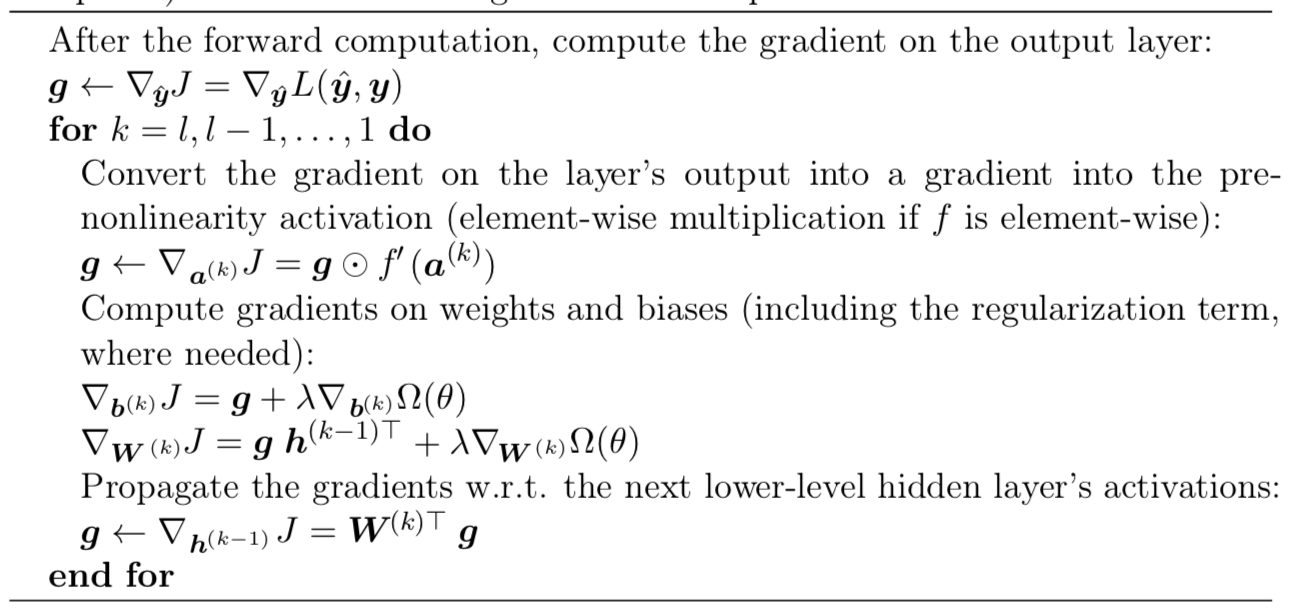
\includegraphics[width=0.6\textwidth]{note_images/backprop_algo.png} %插入图片,[]中设置图片大小,{}中是图片文件名
  \end{figure}

  
\end{document}
